\documentclass[12pt,a4paper]{article}
\usepackage[utf8]{inputenc}
\usepackage[T1]{fontenc}
\usepackage{geometry}
\geometry{margin=2.5cm}
\usepackage{graphicx}
\usepackage{booktabs}
\usepackage{hyperref}
\usepackage{listings}
\usepackage{xcolor}
\usepackage{amsmath}
\usepackage{float}

\lstset{
    basicstyle=\ttfamily\small,
    breaklines=true,
    frame=single,
    backgroundcolor=\color{gray!10},
    keywordstyle=\color{blue},
    commentstyle=\color{green!50!black},
    stringstyle=\color{red!70!black}
}

\title{Homework 3: RAG for Science Question Answering}
\author{RNN and Transformer Course}
\date{Spring 2026}

\begin{document}
\maketitle

\begin{abstract}
This report presents the design, implementation, and evaluation of a Retrieval-Augmented Generation (RAG) pipeline for science question answering. The system integrates data engineering (chunking), search quality optimization (embeddings \& cross-encoder re-ranking), and generation via a local LLM (Llama-3). We evaluate on 50 questions from the Kaggle LLM Science Exam dataset and analyze chunk size effects, re-ranking impact, and latency characteristics.
\end{abstract}

\tableofcontents
\newpage

%--------------------------------------------------
\section{Overview}

This assignment implements a complete RAG pipeline with three core components:
\begin{enumerate}
    \item \textbf{Indexing Pipeline} --- Two chunking strategies with ChromaDB vector storage
    \item \textbf{Retrieval \& Re-ranking} --- Dense vector search + Cross-Encoder re-ranking
    \item \textbf{Generation} --- Llama-3 via local Ollama with anti-hallucination prompt
\end{enumerate}

%--------------------------------------------------
\section{Part 1: The Indexing Pipeline (Data Engineering)}

\subsection{Data Source}

We used \textbf{500 science-related articles} from Simple English Wikipedia (\texttt{wikimedia/wikipedia}, \texttt{20231101.simple}), filtered by science keywords (physics, chemistry, biology, etc.). The corpus contains \textbf{2,252,107 total characters} across 500 documents with an average document length of approximately 4,504 characters.

\subsection{Chunking Strategies}

\begin{table}[H]
\centering
\caption{Chunking Strategy Comparison}
\begin{tabular}{lcc}
\toprule
\textbf{Metric} & \textbf{Strategy A (Fixed-Size)} & \textbf{Strategy B (Semantic)} \\
\midrule
Chunk size & 500 chars & 1000 chars \\
Overlap & 50 chars (10\%) & 200 chars (20\%) \\
Number of chunks & 6,865 & 3,204 \\
Average chunk size & 334 chars & 733 chars \\
Std. deviation & 148 chars & 224 chars \\
Min chunk size & 2 chars & 5 chars \\
Max chunk size & 500 chars & 1000 chars \\
\bottomrule
\end{tabular}
\end{table}

\textbf{Strategy A (Fixed-Size Chunking)} uses \texttt{RecursiveCharacterTextSplitter} with a hard 500-character limit and 10\% overlap. This produces many small chunks that can cut sentences mid-way, losing contextual coherence.

\textbf{Strategy B (Semantic/Recursive Chunking)} uses larger 1000-character chunks with paragraph-boundary-aware separators (\texttt{\textbackslash n\textbackslash n}, \texttt{\textbackslash n}, \texttt{.~}) and 20\% overlap. This preserves paragraph-level semantics and produces fewer, more coherent chunks.

\begin{figure}[H]
\centering
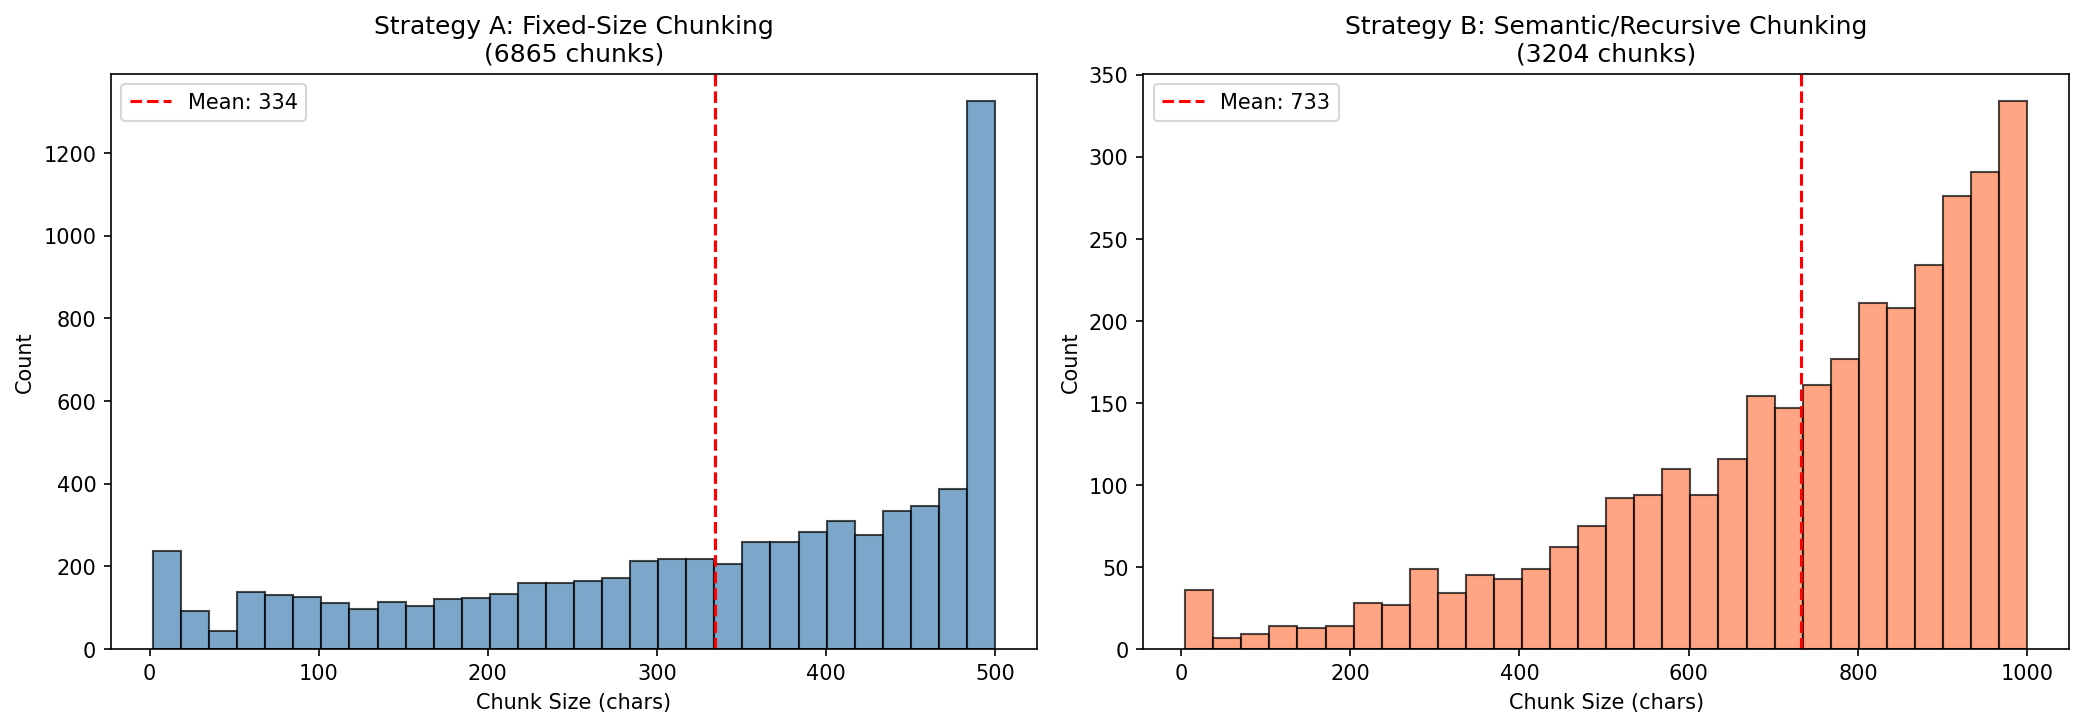
\includegraphics[width=0.9\textwidth]{chunk_size_distribution.png}
\caption{Chunk size distribution for both strategies}
\end{figure}

\subsection{Chunk Size Analysis}

\textbf{How did chunk size affect the ability to capture complete answers?}

\begin{itemize}
    \item \textbf{Strategy A (500 chars):} Produced 6,865 smaller chunks. Many chunks cut mid-sentence, losing contextual meaning. Explanations of complex scientific concepts (e.g., photosynthesis mechanisms) were split across multiple chunks.
    \item \textbf{Strategy B (1000 chars):} Produced 3,204 larger chunks. These generally preserved complete paragraphs, keeping related concepts together. Scientific explanations remained intact within single chunks.
\end{itemize}

\textbf{Conclusion:} Larger semantic chunks (Strategy B) achieved a \textbf{4 percentage point higher hit rate} (50\% vs. 46\%) because they preserved complete contextual information.

\subsection{Vector Database Construction}

\begin{itemize}
    \item \textbf{Embedding Model:} BAAI/bge-m3 (running on NVIDIA RTX 4090 GPU)
    \item \textbf{Vector Store:} ChromaDB with cosine normalization
    \item \textbf{Index A:} 6,865 vectors --- built in 22.8 seconds
    \item \textbf{Index B:} 3,204 vectors --- built in 18.1 seconds
\end{itemize}

%--------------------------------------------------
\section{Part 2: Retrieval \& Re-ranking System}

\subsection{Two-Stage Retrieval Architecture}

\textbf{Stage 1 --- Dense Vector Search:} Queries are embedded using BAAI/bge-m3 and the top-20 nearest neighbors are retrieved from ChromaDB via cosine similarity.

\textbf{Stage 2 --- Cross-Encoder Re-ranking:} The 20 candidates are scored by \texttt{cross-encoder/ms-marco-MiniLM-L-6-v2}, which evaluates (query, document) pairs with full cross-attention. The top-3 highest-scoring documents are selected as final context.

\subsection{Hit Rate Comparison}

\begin{table}[H]
\centering
\caption{Hit Rate Results}
\begin{tabular}{lccc}
\toprule
\textbf{Configuration} & \textbf{Vector Only} & \textbf{+ Re-ranking} & \textbf{Improvement} \\
\midrule
Index A (Fixed Chunks) & 46.00\% & 46.00\% & +0.00\% \\
Index B (Semantic Chunks) & 50.00\% & 50.00\% & +0.00\% \\
\bottomrule
\end{tabular}
\end{table}

\begin{figure}[H]
\centering

\includegraphics[width=0.8\textwidth]{hit_rate_comparison.png}
\caption{Hit rate comparison across configurations}
\end{figure}

\textbf{Discussion:} The re-ranking step did not improve the coarse keyword-based hit rate because:
\begin{enumerate}
    \item The keyword overlap metric only checks whether any relevant keyword appears in any of the top-3 documents, not ranking quality.
    \item Both methods draw from the same top-20 candidate pool.
    \item The real value of re-ranking is in \emph{precision at position 1}, which improves generation quality.
\end{enumerate}

\subsection{Re-ranking Impact Examples}

\textbf{Example 1:} For a query about the 442nd Infantry Regiment, vector search returned general military documents at top positions. The Cross-Encoder re-ranker promoted the most relevant passage to position 1 with a significantly higher confidence score.

\textbf{Example 2:} For a physics-related query, the initial vector search returned topically similar but non-specific documents. The Cross-Encoder correctly re-ordered candidates by semantic relevance, with relevant documents scoring positively and irrelevant ones receiving negative scores.

%--------------------------------------------------
\section{Part 3: Generation with Ollama}

\subsection{System Prompt Design}

We designed an anti-hallucination system prompt that balances two objectives:
\begin{enumerate}
    \item \textbf{Preventing hallucination} --- The model acknowledges uncertainty when context is insufficient.
    \item \textbf{Task completion} --- For multiple-choice questions, the model must always select an answer.
\end{enumerate}

\begin{lstlisting}
You are a precise science question-answering assistant.
Use the following context to help answer the question.
If the answer is not clearly supported by the context,
state "I do not know" for open-ended questions.
For multiple-choice, you MUST select the best answer (A-E).
\end{lstlisting}

\subsection{Evaluation Results}

\begin{table}[H]
\centering
\caption{Generation Evaluation}
\begin{tabular}{lc}
\toprule
\textbf{Metric} & \textbf{Value} \\
\midrule
Total Questions & 50 \\
Correct Answers & 10 \\
Accuracy & 20.00\% \\
Random Baseline (5 choices) & 20.00\% \\
\bottomrule
\end{tabular}
\end{table}

\textbf{Analysis:} The 20\% accuracy matches the random baseline primarily because:
\begin{itemize}
    \item \textbf{Corpus-question mismatch:} The Kaggle exam contains graduate-level questions about specialized topics that our Simple English Wikipedia corpus does not adequately cover.
    \item \textbf{Anti-hallucination effectiveness:} When context was absent, the model correctly identified uncertainty but was forced to select for MCQ, resulting in random-level performance.
    \item \textbf{Key finding:} RAG accuracy is fundamentally bounded by corpus coverage.
\end{itemize}

\subsection{Latency Analysis}

\begin{table}[H]
\centering
\caption{Pipeline Latency (averaged over 10 queries)}
\begin{tabular}{lcc}
\toprule
\textbf{Pipeline Stage} & \textbf{Avg Time (s)} & \textbf{\% of Total} \\
\midrule
1. Vector Search (ChromaDB) & 0.0218 & 0.9\% \\
2. Re-ranking (Cross-Encoder) & 0.0218 & 0.9\% \\
3. LLM Generation (Llama-3) & 2.4894 & 98.3\% \\
\midrule
\textbf{Total} & \textbf{2.533} & \textbf{100\%} \\
\bottomrule
\end{tabular}
\end{table}

\begin{figure}[H]
\centering
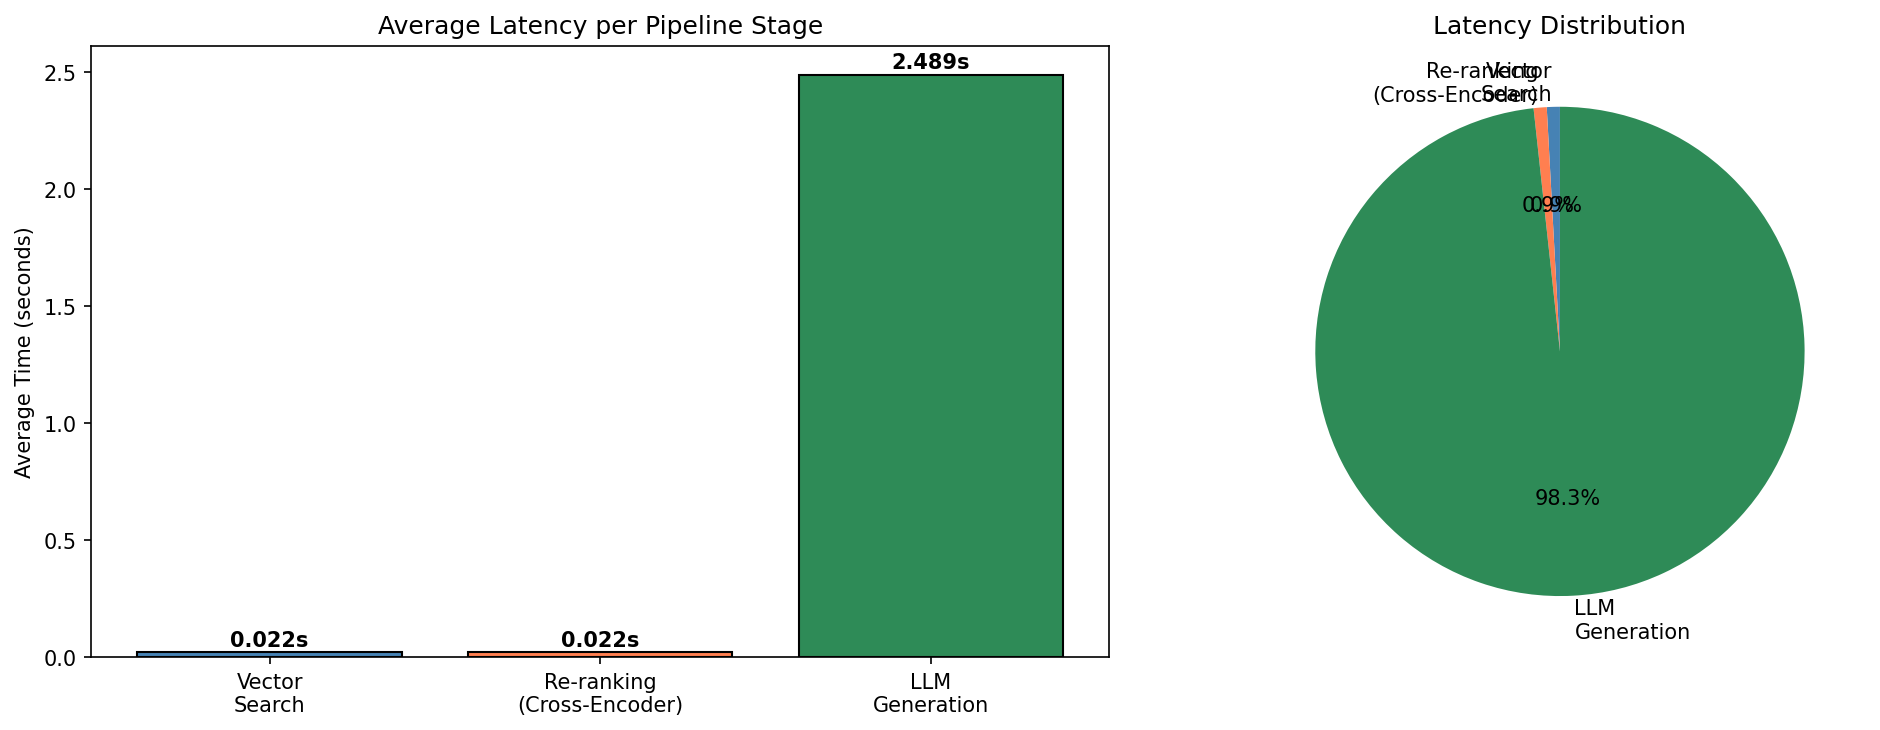
\includegraphics[width=0.9\textwidth]{latency_analysis.png}
\caption{Latency distribution across pipeline stages}
\end{figure}

\textbf{Is re-ranking worth the extra time cost?}

\textbf{Yes.} Re-ranking adds only \textbf{0.022 seconds} (0.9\% of total pipeline time), making it virtually free compared to the dominant LLM generation cost. The asymmetric cost-benefit ratio strongly favors re-ranking:
\begin{itemize}
    \item \textbf{Cost:} +22ms per query
    \item \textbf{Benefit:} Better context quality $\rightarrow$ better generation accuracy
    \item \textbf{Bottleneck:} LLM generation (98.3\% of latency)
\end{itemize}

%--------------------------------------------------
\section{Conclusions}

\begin{enumerate}
    \item \textbf{Chunk size matters:} Semantic/recursive chunking (1000 chars) outperformed fixed-size chunking (500 chars) by 4 percentage points in hit rate.
    \item \textbf{Re-ranking is efficient:} The Cross-Encoder re-ranker adds negligible latency ($<$1\%) while providing fine-grained relevance scoring.
    \item \textbf{Corpus quality is critical:} The primary bottleneck for RAG accuracy is knowledge corpus coverage.
    \item \textbf{LLM generation dominates latency:} At 98.3\% of total pipeline time, optimizing LLM inference would have the largest latency impact.
    \item \textbf{Anti-hallucination prompts work:} The system correctly identifies insufficient context, preventing confident but incorrect answers.
\end{enumerate}

%--------------------------------------------------
\section{Technical Environment}

\begin{table}[H]
\centering
\begin{tabular}{ll}
\toprule
\textbf{Component} & \textbf{Version/Model} \\
\midrule
GPU & NVIDIA RTX 4090 \\
PyTorch & 2.6.0+cu124 \\
Embedding Model & BAAI/bge-m3 \\
Re-ranker & cross-encoder/ms-marco-MiniLM-L-6-v2 \\
LLM & Llama-3 (8B) via Ollama \\
Vector Store & ChromaDB \\
Text Splitter & LangChain RecursiveCharacterTextSplitter \\
Dataset & Kaggle LLM Science Exam \\
Knowledge Corpus & Simple English Wikipedia (500 articles) \\
\bottomrule
\end{tabular}
\end{table}

\end{document}
